%\mbox{}
%\thispagestyle{empty}
%\newpage
\thispagestyle{plain}
\section{Computational modeling}
\indent

For modeling of thermoset polymers we have used three methods of numerical solution. Firstly, the Drucker-Prager plasticity model used to simulate the mechanical behavior. The implementation follows the approach presented in \cite{geofem}. More specifically, the robust object-oriented finite element (FE) solver MARS \cite{mars} is utilized for the implementation. Therefore, the curing model for polymers already implemented in MARS can be later utilize to account for the evolving of material properties caused by the change of curing degree.

\subsection{Finite element method}
\indent

Finite element method (FEM) is a numerical solution used for the simulation of stresses, strains, natural frequency, heat transition, electromagnetic effects, flow of fluids, etc., on a created physical model. The main principle is the discretization of continuum into finite number of elements. FEM is typically used to simulate the realistic behavior of structures or for determination of critical regions of structures. Through principles of this method were developed in first half of twentieths century, its massive expansion occurred with succession of a modern computer technologies due to necessary high computing power. The detail of description of FEM is out of the scope of this thesis and can be found in \cite{dhatt2012finite}. 
\begin{comment}
	content

\newpage
\subsection{Vectors and matrices}
\indent

Before describing individual constitutive models is necessary to define the following matrices and vectors frequently used in the Drucker-Prager model:

\begin{equation}
	\boldsymbol{m} = \lbrace 1/3,1/3,1/3\rbrace ^T,
\end{equation}


\begin{equation}
	\boldsymbol{P} = \mqty[	2/3 & -1/3 & -1/3 & 0 & 0 & 0\\ 
				-1/3 & 2/3 & -1/3 & 0 & 0 & 0\\
				-1/3 & -1/3 & 2/3 & 0 & 0 & 0\\
				0 & 0 & 0 & 2 & 0 & 0\\
				0 & 0 & 0 & 0 & 2 & 0\\
				0 & 0 & 0 & 0 & 0 & 2\\],	\boldsymbol{Q} = \mqty[	1 & 0 & 0 & 0 & 0 & 0\\
				0 & 1 & 0 & 0 & 0 & 0\\
				0 & 0 & 1 & 0 & 0 & 0\\
				0 & 0 & 0 & 1/2 & 0 & 0\\
				0 & 0 & 0 & 0 & 1/2 & 0\\
				0 & 0 & 0 & 0 & 0 & 1/2\\],
\end{equation}


\end{comment}


\subsection{Drucker-prager model of plasticity}\label{sec:drucker-prager_introduction}
\indent

Drucker-Prager (DP) model of plasticity can be seen as the extension of the von Mises model and enhances it by including mean stress into the yield surface equation. Unlike Mohr-Coulomb (MC) model, the Drucker-Prager yield criterion is smooth and in space of the principal stresses have form of cylindrical cone, see Fig. \ref{obr:F1}. In current implementation parameters are adjusted to fit or inscribe to Mohr-Coulomb model. The main advantage of DP over MC is the simplification of return to the yield surface because of its smoothness. As already mentioned, the definition and the calculation of Drucker-Prager model in this thesis is based on \cite{geofem}.   

\begin{figure}[h!]
	\centering	
	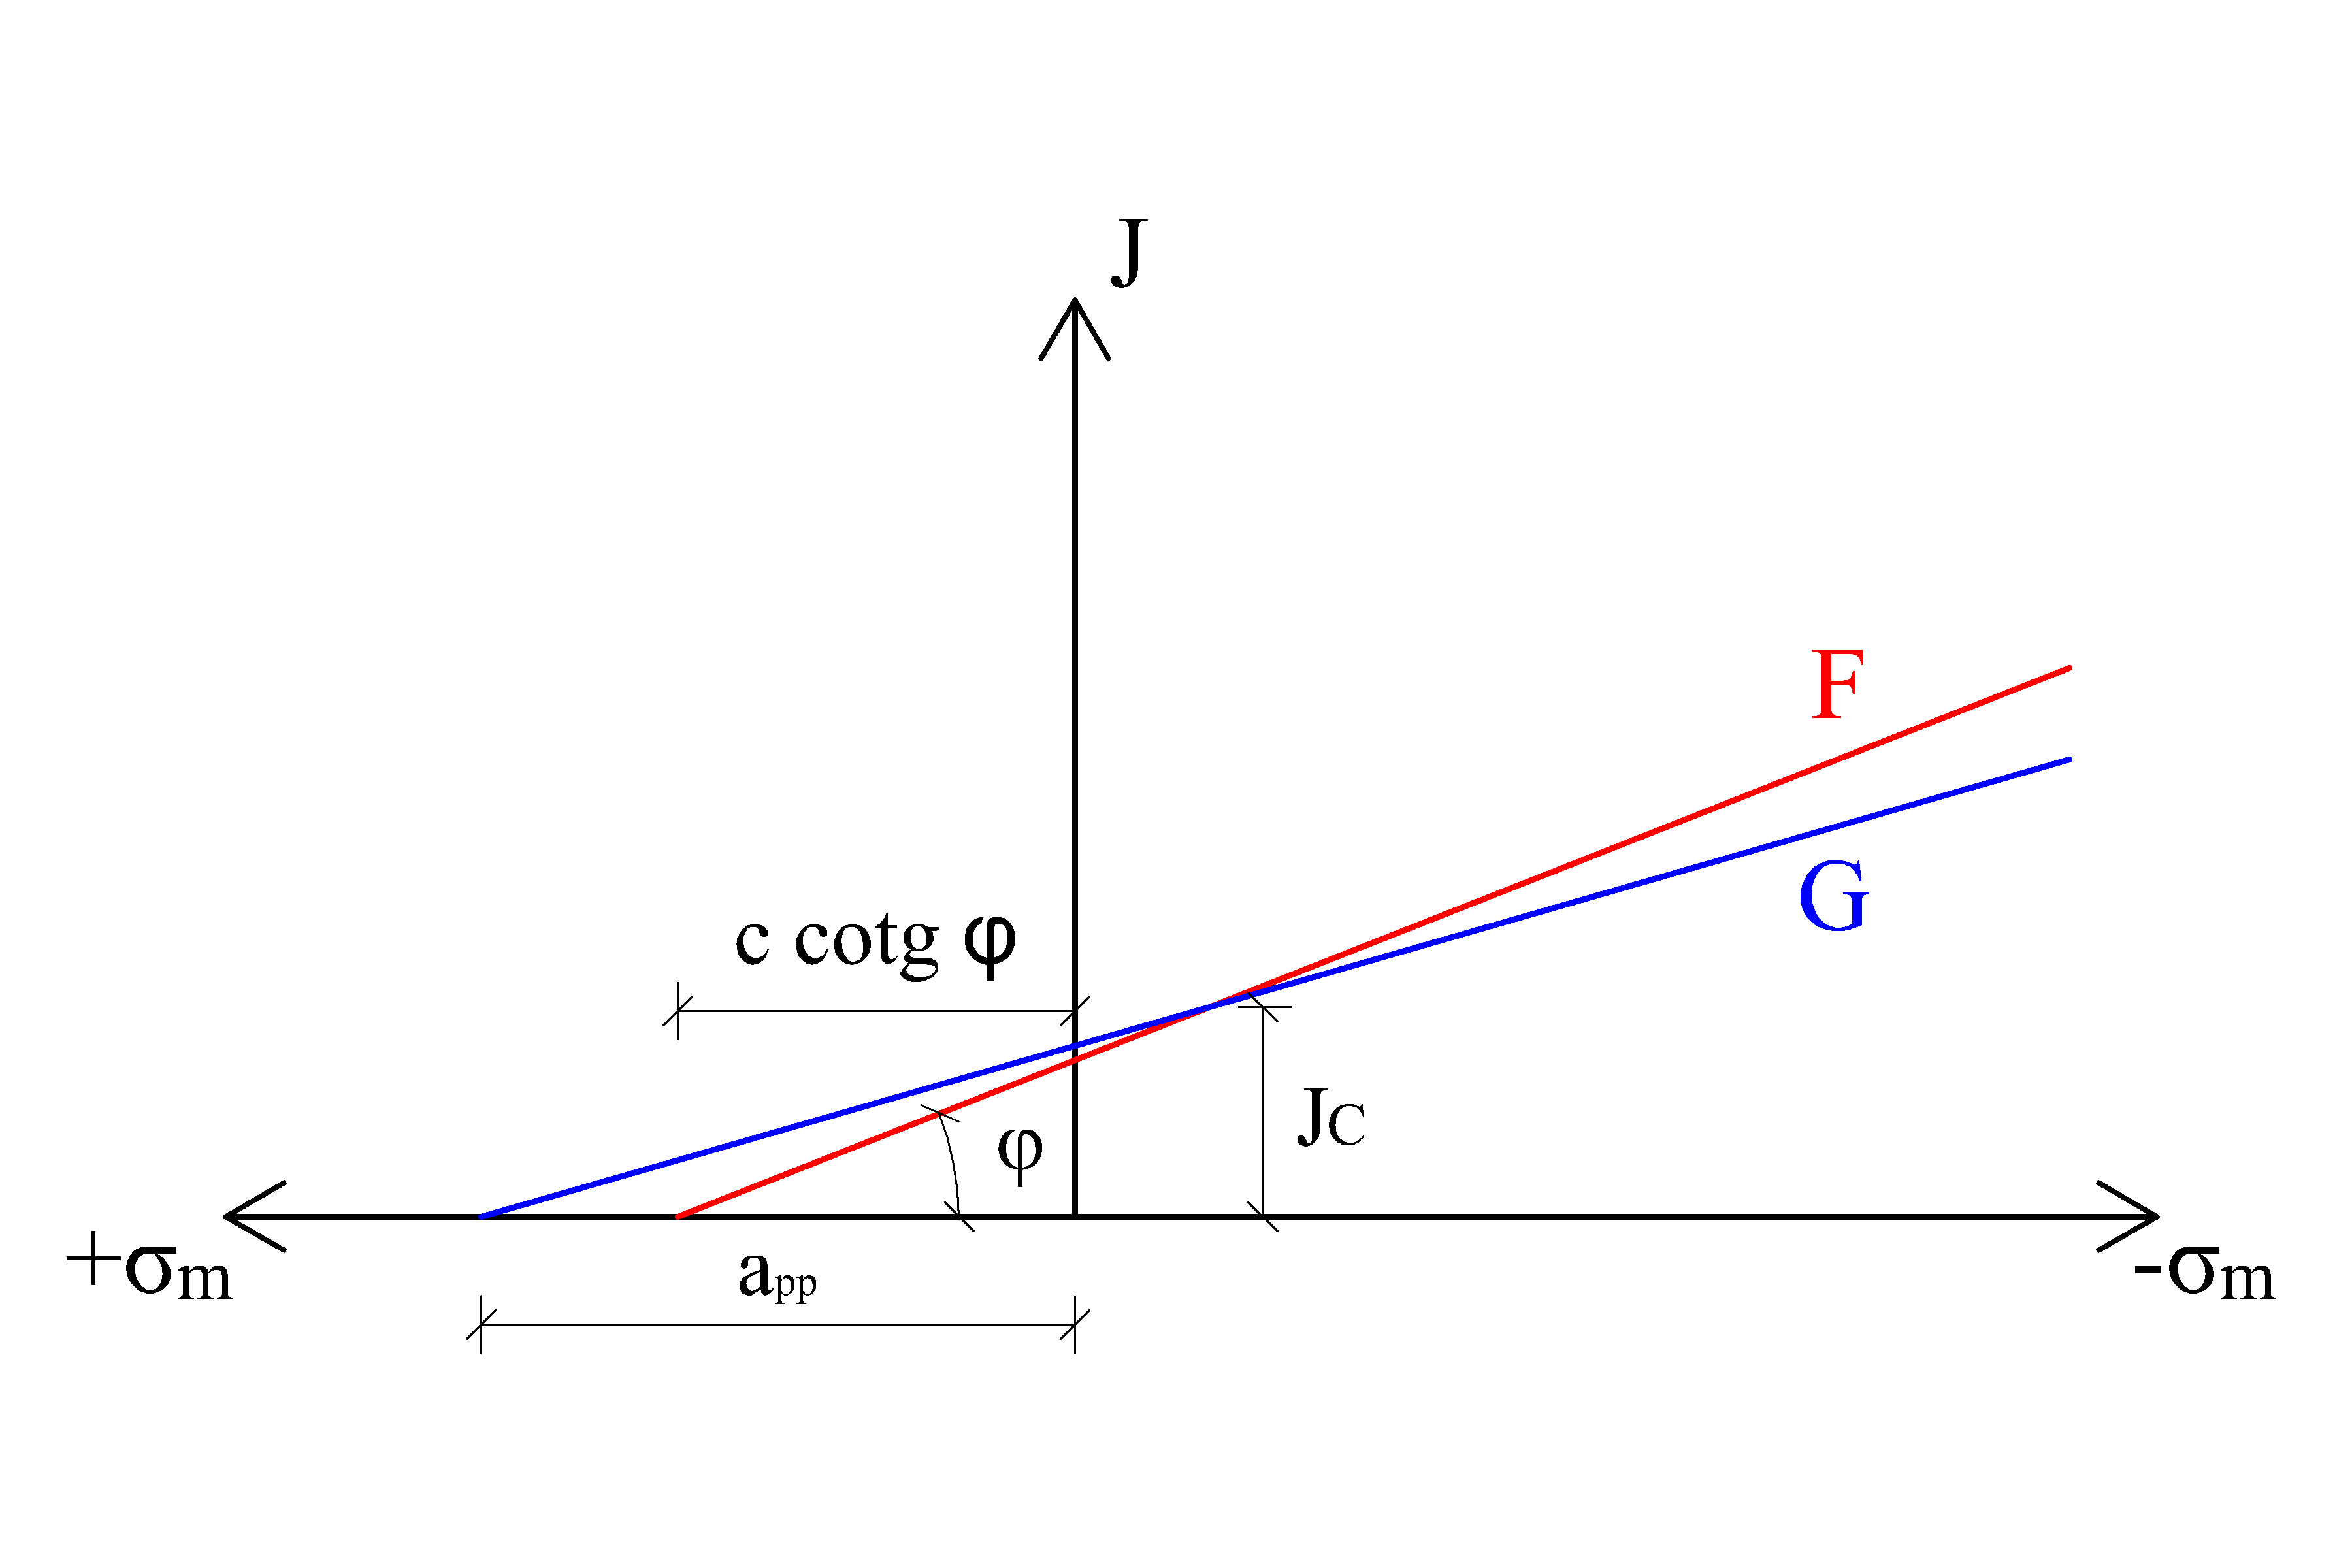
\includegraphics[width=0.7\textwidth, angle=0]{obrazky/drucker_prager_meridian_my.png}
	\caption[Drucker-Prager yield criterion on meridian plane]{Drucker-Prager yield criterion in meridian plane \cite{geofem}: F is yield function; G means plastic potential function.} \label{obr:M1}
\end{figure}

\subsubsection{Drucker-Prager yield surface}\label{sec:drucker-prager_yield_criterion}
\indent

Drucker-Prager yield criterion equation describes boundary, where material ceases to behave elastically and becomes elasto-plastic and can be written as  

\begin{equation}\label{eq:f_yc}
	F(\sigma) = J + (\sigma_m-c(\kappa_{1}) \cot \varphi(\kappa_{2}) )M_{JP}(\varphi(\kappa_{2})) = 0,
\end{equation}
where $J$ is a square root of the second invariant of the deviatoric stress, $\sigma_m$ is the mean stress with the form 
 
\begin{equation}\label{eq:f_J_sigM}
	J = \sqrt{\dfrac{1}{6} \left[(\sigma_{11}-\sigma_{22})^{2} + (\sigma_{11}-\sigma_{33})^{2} + (\sigma_{22}-\sigma_{33})^{2}\right] + \tau_{12}^{2} + \tau_{13}^{2}+ \tau_{23}^{2}},
\end{equation}


\begin{equation}\label{eq:f_sigM}
	\sigma_m = \dfrac{\sigma_{11} + \sigma_{22} + \sigma_{33}}{3},
\end{equation}
and $M_{JP}$ is used for approximation to the Mohr-Coulomb model, which can be done with more forms dependent on point, which is intended to approximate. Three different Drucker-Prager cones are in the Fig \ref{obr:F1}. The first one, red circle, touches Mohr-Coulomb yield criterion at $\theta = 30^\circ$ (triaxial compression) with $M_{JP}$ defined as

\begin{figure}[h!]
	\centering	
	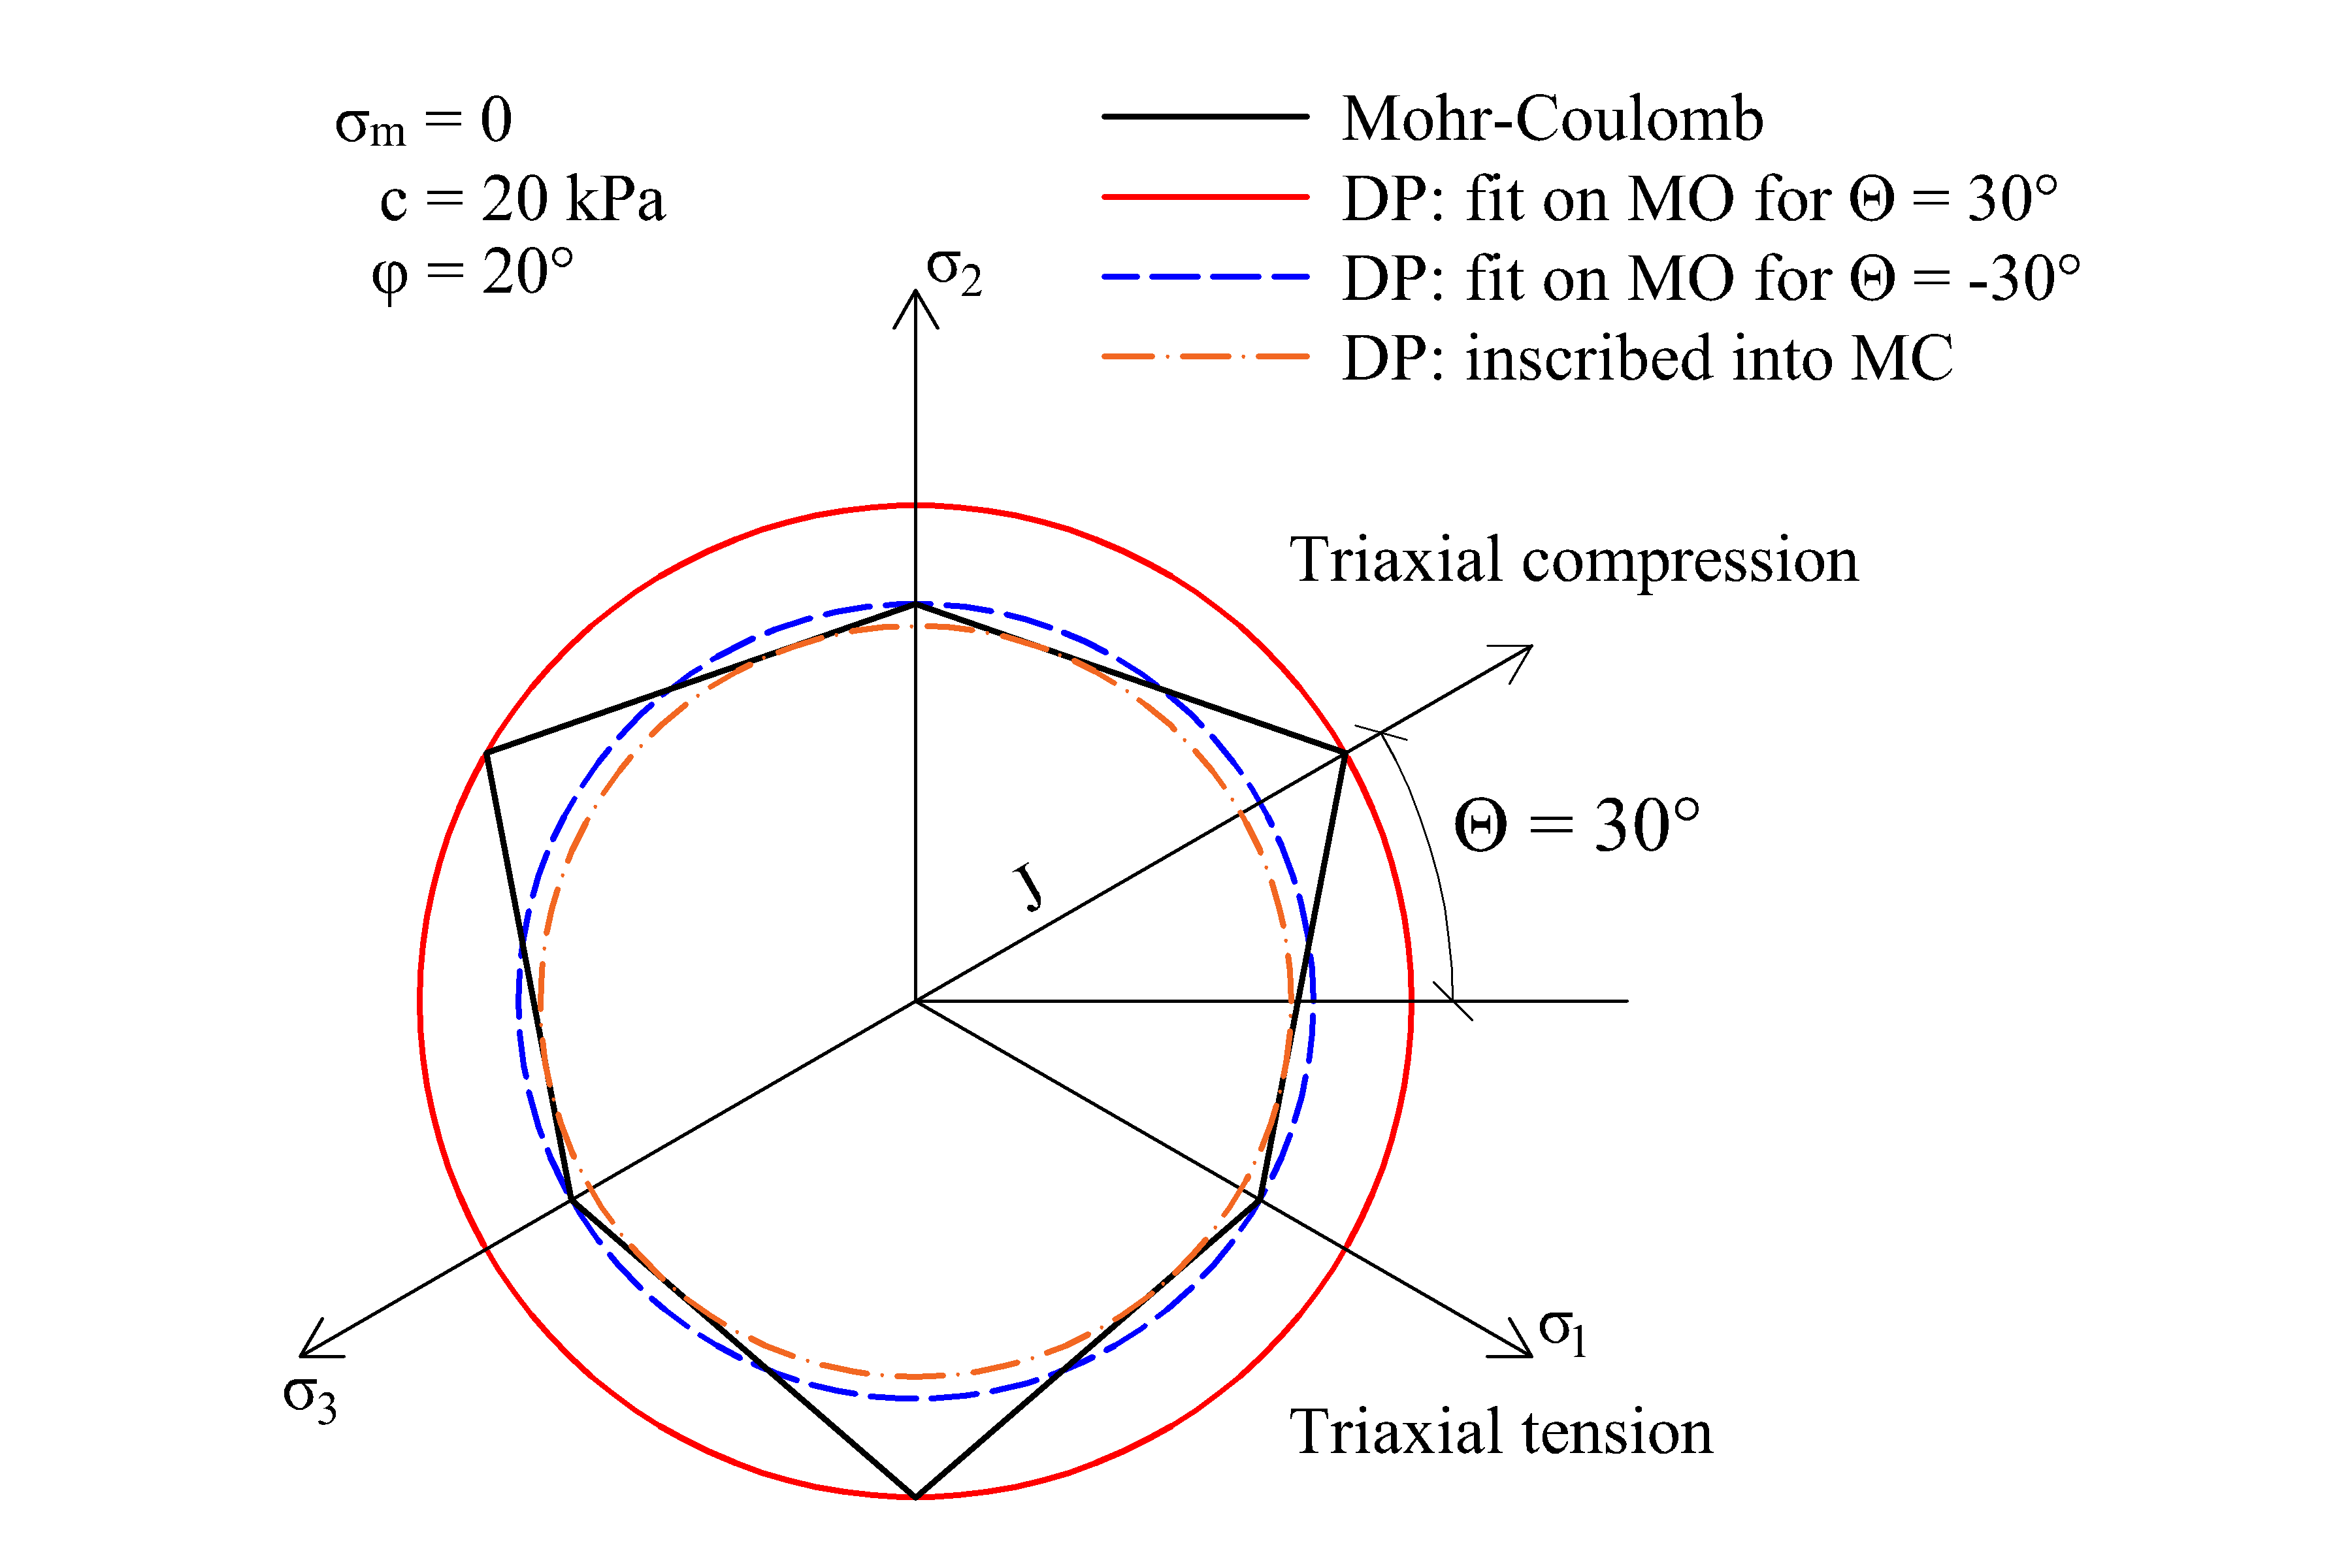
\includegraphics[width=0.8\textwidth, angle=0]{obrazky/drucker-prager_eng.png}
	\caption[Drucker-Prager and Mohr-Coulomb model]{Drucker-Prager and Mohr-Coulomb yield criterion in space of principal stresses \cite{geofem}. \label{obr:F1}}
\end{figure}



\begin{equation}\label{eq:f_Mjp_30}
	M_{JP}^{\theta=30^\circ} = \dfrac{2\sqrt{3}\sin\varphi}{3-\sin \varphi},
\end{equation}
where $\varphi$ is the angle of internal friction. The second, blue circle, match the Mohr-Coulomb model at  $\theta = -30^\circ$ (triaxial tension), can be obtained as

\begin{equation}\label{eq:f_Mjp_-30}
	M_{JP}^{\theta=-30^\circ} = \dfrac{2\sqrt{3}\sin\varphi}{3+\sin \varphi},
\end{equation}
and the last, the green circle, is inscribed, and can be determined by

\begin{equation}\label{eq:f_Mjp_i}
	M_{JP}^{ins} = \dfrac{\sin(\varphi)}{\cos(\theta)^{ins}-\frac{\sin(\theta^{ins})\sin(\varphi)}{\sqrt{3}}},
\end{equation}

\begin{equation}\label{eq:f_theta}
	\theta^{ins} = \arctan{\frac{\sin{\varphi}}{\sqrt{3}}}.
\end{equation}

The Drucker-Prager model is not defined just by the yield function $F$ but also $G$, which is the plastic potential function, see Fig. \ref{obr:M1}. $G$ defines vector of return to the yield of plasticity, when it is overpassed, and can be written in the form 

\begin{equation}\label{eq:G}
	G = J + \left[ \sigma_m - a_{pp} \right] M_{JP}^{PP} = 0,
\end{equation}
where $a_{pp}$ follows from Fig. \ref{obr:M1}. When matching Eqs. (\ref{eq:f_yc}) and (\ref{eq:G}) for the current value of stress $\sigma$, result has the form

\begin{equation}\label{eq:app}
	a_{pp} = - \sigma_m^c + ( \sigma_m^c - c\cot\varphi) \dfrac{M_{JP}}{M_{JP}^{PP}}
\end{equation} 
By substituting $a_{pp}$ into the plastic potential function (\ref{eq:G}), we arrive at

\begin{equation}\label{eq:plastic_potential}
	G = J + \left[ \sigma_m - - \sigma_m^c + ( \sigma_m^c - c\cot\varphi) \dfrac{M_{JP}}{M_{JP}^{PP}} \right] M_{JP}^{PP} = 0,
\end{equation}
where $M_{JP}^{PP}$ is the gradient of the plastic potential function in $J-\sigma_m$ space (Fig \ref{obr:M1}). When functions of plastic potential and yield function  $M_{JP}^{PP}=M_{JP}$, Drucker-Prager model becomes associated. $M_{JP}^{PP}$  can be referred as the angle of dilatation $\psi$, and can be substituted for $\varphi$ in Equations (\ref{eq:f_Mjp_30})-(\ref{eq:f_theta}).
 
\subsubsection{Hardening and softening modulus}
\indent

 In Drucker-Prager model implemented derivation of hardening/softening modulus is inspired by the von Mises. To that end, we choose multi-linear form of the hardening/softening law for the cohesion $c$ and the angle of internal friction $\varphi$, as shown in Fig. \ref{obr:H}, where the dependence of $c$ and $\varphi$ on the deviatoric plastic strain $E_d^{pl}$ can be seen. Though the components of vector $\kappa$ may vary for each of the two strength parameters, in the present formulation a single hardening parameter is assumed 
 
\begin{equation}\label{eq:kappa}
	\kappa = \kappa_{1} = \kappa_{2} = E_d^{pl}.
\end{equation}

\begin{figure}[h!]
	\centering	
	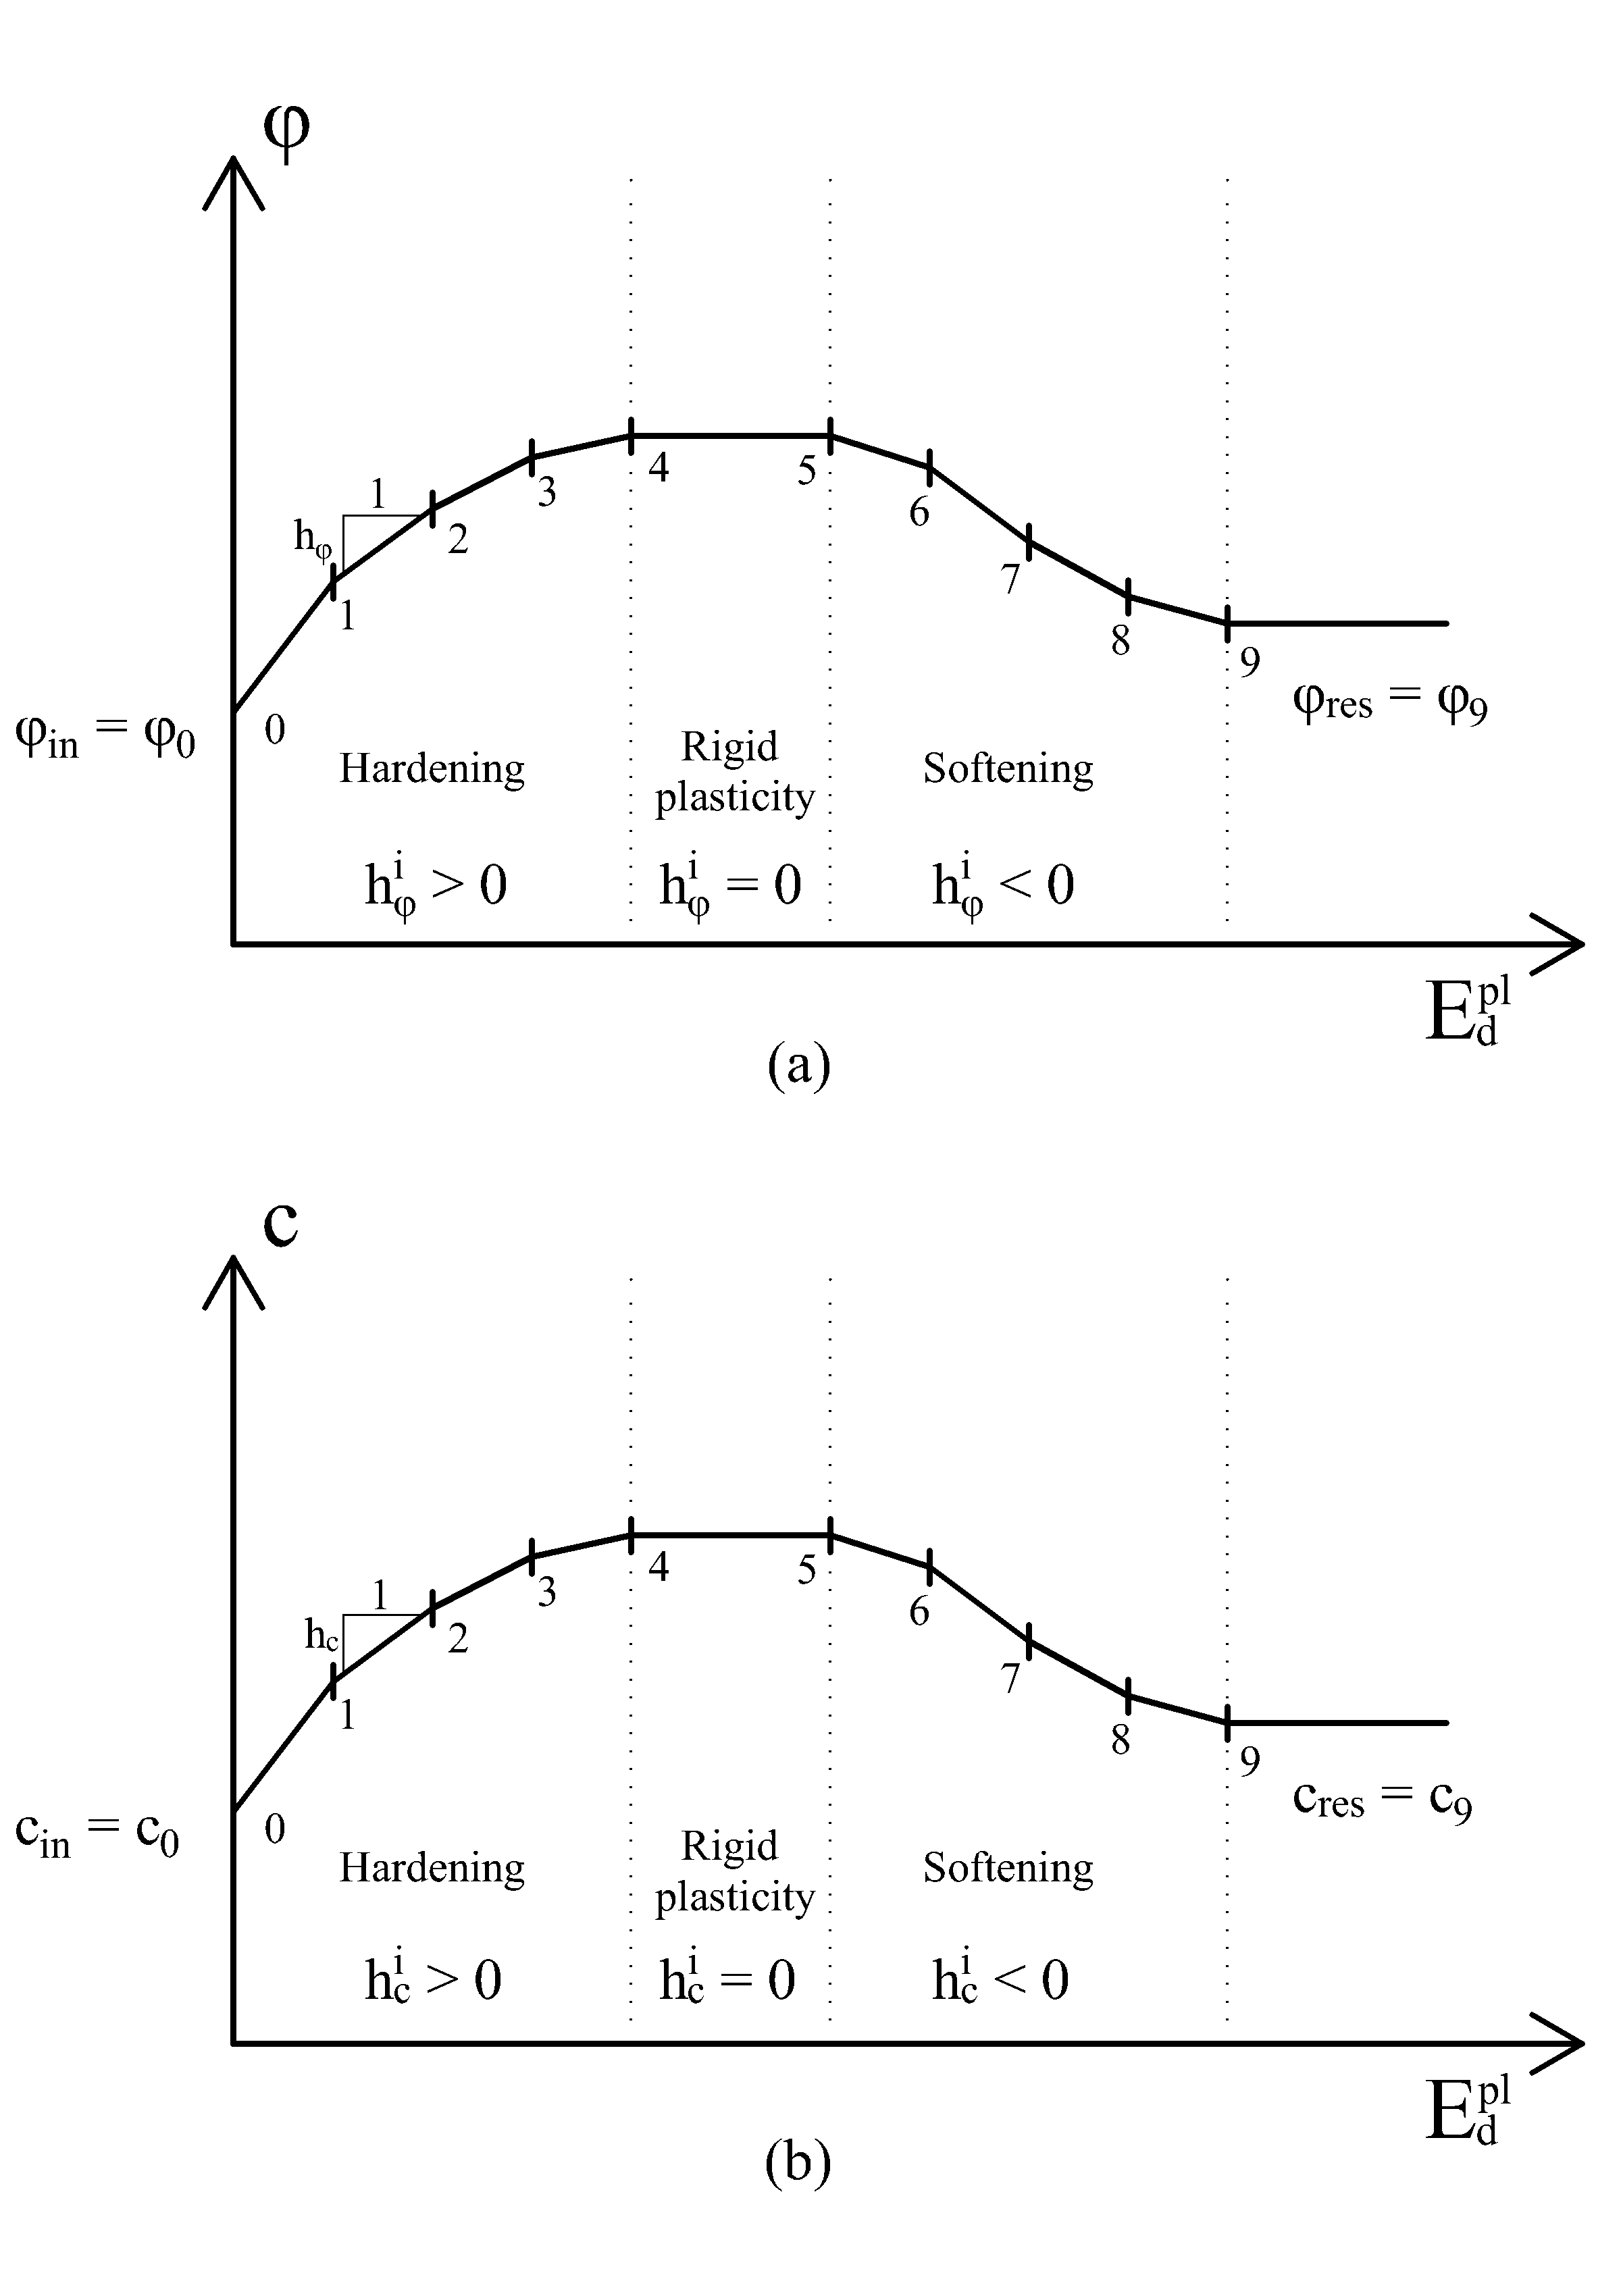
\includegraphics[width=0.70\textwidth, angle=0]{obrazky/hardening_softening_modulus_my.png}
	\caption[Hardening and softening modulus]{Hardening and softening modulus \cite{geofem}: $c_{in}$ and $c_{res}$, respective $\varphi_{in}$ and $\varphi_{res}$ represent initial and residual values of $c$ and $\varphi$.} \label{obr:H}
\end{figure}
 
Multi-linear formulation assumes that if $n^{th}$ interval in the Fig. \ref{obr:H} is active, then the current strenght parameters can be determined by

\begin{equation}\label{eq:c}
	c = c^{n-1} + h_c^n \left( E_d^{pl} -(E_d^{pl})^{n-1} \right),
\end{equation}

\begin{equation}\label{eq:phi}
\varphi = \varphi^{n-1} + h_\varphi^n\left( E_d^{pl} - (E_d^{pl})^{n-1} \right),
\end{equation}
where $h_c^n$ and $h_\varphi^n$ are the hardening/softening moduli for $c$ and $\varphi$ and can be written in the form


\begin{equation}\label{eq:h_c}
	h_c^n = \dfrac{c^n-c^{n-1}}{(E_d^{pl})^{n}-(E_d^{pl})^{n-1}}
\end{equation}

\begin{equation}\label{eq:h_phi}
 	\varphi_c^n = \dfrac{\varphi^n-\varphi^{n-1}}{(E_d^{pl})^{n}-(E_d^{pl})^{n-1}}
\end{equation}

Following \cite{geofem}, the hardening modulus can be determined by

\begin{equation}\label{eq:H_first}
	H = \left(-\dfrac{\partial F}{\partial \kappa}\right)^T \dfrac{\partial \kappa}{\partial \lambda},
\end{equation}
and referring to Fig. \ref{obr:H} and using Eq. (\ref{eq:H_first}) the hardening/softening modulus $H$ assumes the form 

\begin{equation}\label{eq:H}
	H = - \pdv{F}{c} \dv{c}{E_d^{pl}} \dv{E_d^{pl}}{\lambda} - \pdv{F}{\varphi} \dv{\varphi}{E_d^{pl}} \dv{E_d^{pl}}{\lambda},
\end{equation}
where

\begin{align}
\pdv{F}{\varphi}& = \dfrac{c}{\sin^2\varphi} M_{JP} + (\sigma_m - c\cot \varphi) \dv{M_{JP}}{\varphi},\label{eq:F/phi}\\
\dv{F}{c}& = - \cot \varphi M_{JP},\\
\dv{c}{\kappa}& = \dv{c}{E_d^{pl}} = h_c,\\
\dv{\varphi}{\kappa}& = \dv{\varphi}{E_d^{pl}} = h_\varphi
\end{align}
Derivations of $M_{JP}$ with respect to $\varphi$ for selected values of $\theta$ are

\begin{align}
	\dv{M_{JP}^{ins}}{\varphi}					& = \dfrac{3\sqrt{3}\cos \varphi}{(3 + \sin^2 \varphi)^{\frac{3}{2}}},\\
	\dv{M_{JP}^{\theta = \ang{-30}}}{\varphi}	& = \dfrac{6\sqrt{3}\cos \varphi}{(1-\sin \varphi)^2},\\
	\dv{M_{JP}^{\theta = \ang{30}}}{\varphi}	& = \dfrac{6\sqrt{3}\cos \varphi}{(1+\sin \varphi)^2}.
\end{align}
By accepting the strain hardening approach, we can write

\begin{align}\label{eq:dkappa}
	\dd\kappa& = \dd E_d^{pl} = \sqrt{2(\Delta e^{pl})^T \Delta e^{pl} } = \dd \lambda \Rightarrow \dv{E_d^{pl}}{\lambda} = 1,
\end{align}
where  $\Delta e^{pl}$ stands for the increment of deviatoric plastic strain vector. With final substitution of Eq. (\ref{eq:F/phi})-(\ref{eq:dkappa}) back into Eq. (\ref{eq:H}), result is searched form of the hardening/softening modulus as

\begin{equation}\label{eq:H_final}
	H = h_c \cot\varphi M_{JP} - h_\varphi \left[ \dfrac{c}{\sin^2 \varphi} M_{JP} + (\sigma_m - c \cot \varphi) \dv{M_{JP}}{\varphi} \right].
\end{equation}


\subsubsection{Calculation procedure and implementation}\label{sec:drucker-prager_count}
\indent
Total stress can be calculated as 
\begin{equation}\label{eq:f_sigma}
\sigma = \text{\textbf{D}}^{el} \varepsilon_{el},
\end{equation}
where \textbf{D}$^{el}$ is an ordinary isotropic stiffness matrix and $\varepsilon_{el}$ is a elastic deformation. Calculation is performed in explicit software \cite{mars}, so model is implemented in the incremental form. Then Eq. \ref{eq:f_sigma} is modified as

\begin{equation}\label{eq:f_sigma1}
	\sigma^{n+1} = \sigma^n+ \text{\textbf{D}}^{el} \mathrm{d} \varepsilon_{el}.
\end{equation}

During numerical procedure, the trial stress $ \sigma_{tr}^{n+1} = \sigma^n + \textbf{D}^{el}\dd\varepsilon$, where $\dd\varepsilon$ is a strain increment, is calculated at the beginning of each step. If Eq. (\ref{eq:f_yc}) is satisfied, strains and stresses are stored, and calculation continues with next deformation increment. If the yield function is violated, the material behavior changes from the basic elastic to the elasto-plastic with hardening. Due to higher amount of the variables, which describe return to the yield surface of plasticity, is necessary to implement the Jacobian matrix\footnote{Matrix of partial derivations}. There are four material parameters driving the return to yield surface of plasticity:

\begin{itemize}
	\item $\Delta\lambda$ - Coefficient of plastic flow,
	\item $c$ - Cohesion,
	\item  $\varphi$ - Angle of friction,
	\item $\psi$ - Angle of dilatation.
\end{itemize}

Before describing the Jacobian matrix, we need to define basic equations, to be used for the definition of all variables. Assume that the plastic strain increment have the form 

\begin{equation}
	\dd \varepsilon^{pl} = \Delta \lambda \pdv{G}{\sigma},
\end{equation}
and with accepting this flow rule, increments of yield respective plastic strain have the form 

\begin{align}
	\dd \varepsilon_\nu^{pl} &= \dd \lambda \pdv{G}{\sigma_m} = \Delta \lambda M_{JP}^{PP} \sin \psi,\\
	%\dd e^{pl} &= \dd \lambda \pdv{G}{s} = \dd \lambda \dfrac{\text{\textbf{G}}^{-1}s}{2J}\text{ where } s = \text{\textbf{PQ}}\sigma,\\
	\dd E_{d}^{pl} &= \dd \lambda \pdv{G}{J} = \Delta \lambda,
\end{align}
which further allows writing the corresponding stresses at the end of the $i+1$ load increment as  

\begin{align}
	\sigma_m^{i+1} &= \sigma_m^{tr} - K M_{JP}^{PP} (\sin \psi^{i+1}) \Delta \lambda,\\
	%s^{i+1} &= s^{tr} - 2\mu \Delta \lambda\dfrac{s^{i+1}}{2J^{i+1}} = \dfrac{s^{tr}}{1 + \dfrac{\mu \Delta \lambda}{J^{i+1}}} = s^{tr} \left( 1 - \dfrac{\mu \Delta \lambda}{J^{tr}}   \right),\\
	J^{i+1} &= J^{tr} + \mu \Delta \lambda,
\end{align}
where $K$ is the bulk modulus and $\mu$ represent the elastic shear modulus to avoid misinterpretation with the plastic potential function. Then the Jacobian matrix can be already defined.

\begin{itemize}
	\item Primary variables
	
	\begin{equation}
		\lbrace \mathbf{a} \rbrace ^T = \lbrace \Delta \lambda, c^{i+1}, \varphi^{i+1}, \psi^{i+1} \rbrace.
	\end{equation}
	
	\item Residuals
	\begin{equation}
		\lbrace \mathbf{r} \rbrace^T =  \lbrace \mathcal{F}, \mathcal{C}, \mathrm{\Phi}, \mathrm{\Psi} \rbrace,
	\end{equation}
	where \begin{align}
		\mathcal{F} &= \overbrace{J^{tr}-\mu\Delta\lambda}^{J^{i+1}} + [\overbrace{\sigma_m^{tr}-K M_{JP}^{PP}(\sin \psi^{i+1})\Delta\lambda}^{\sigma_m^{i+1}}-c^{i+1}\cot\varphi^{i+1}]M_{JP}(\sin\varphi^{i+1}),\label{eq:f_yc_lam}\\
		\mathcal{C} &= c^{i+1} - \hat{c} = 0,\label{eq:C_jac}\\
		\mathrm{\Phi} &= \varphi^{i+1} - \hat{\varphi} = 0,\label{eq:phi_jac}\\
		\mathrm{\Psi} &= \psi^{i+1} - \hat{\psi} = 0.
	\end{align}
	Variables $\hat{c}$ and $\hat{\varphi}$ follows Eq.(\ref{eq:c}) and (\ref{eq:phi}) and the current value of dilatation angle $\hat{\psi}$ can be, with help of Rowe's dilatation theory in triaxial compression, written as
	\begin{equation}
		\sin \hat{\psi} = \dfrac{\sin \varphi^{i+1} - \sin \varphi_{cv}}{1 - \sin \varphi^{i+1} \sin \varphi_{cv}},
	\end{equation}
	where $\varphi_{cv}$ is a constant-volume friction angle.
	
	\item Local Newton-Raphson method
	\begin{equation}\label{eq:newton_raphson}
		\lbrace a^{i+1} \rbrace _{k+1} = \lbrace a^{i+1}_k \rbrace - [\text{\textbf{H}}]^{-1} \lbrace r \rbrace_k 
	\end{equation}
	
	\item Jacobian matrix $[\textbf{H}]$
	\begin{equation}
		[\text{\textbf{H}}] = \mqty[\pdv{J}{\Delta \lambda} \pdv{\mathcal{F}}{\sigma_m} \pdv{\sigma_m}{\Delta \lambda} & \pdv{\mathcal{F}}{c} & \pdv{\mathcal{F}}{\varphi} + \pdv{\mathcal{F}}{M_{JP}} \pdv{M_{JP}}{\sin \varphi} & \pdv{\mathcal{F}}{M_{JP}^{PP}} \pdv{M_{JP}^{PP}}{\sin \psi}\\
		\pdv{\mathcal{C}}{\hat{c}} \pdv{\hat{c}}{\Delta \lambda} & \pdv{\mathcal{C}}{c} & 0 & 0\\
		\pdv{\mathrm{\Phi}}{\sin \hat{\varphi}} \pdv{\hat{\varphi}}{\Delta \lambda} & 0 & \pdv{\mathrm{\Phi}}{\sin \varphi} & 0 \\
		0 & 0 & \pdv{\mathrm{\Psi}}{\sin \hat{\psi}} \pdv{\sin \hat{\psi}}{\sin \varphi} & \pdv{\mathrm{\Psi}}{\sin \psi}]
	\end{equation}
	where partial derivations are
	\begin{align}
		&\pdv{J}{\Delta \lambda} \pdv{\mathcal{F}}{\sigma_m} \pdv{\sigma_m}{\Delta \lambda}  = -\mu - K M_{JP}^{PP}M_{JP},\\
		&\pdv{\mathcal{F}}{c} = -M_{JP}\tan\varphi,\\
		&\pdv{\mathcal{F}}{\varphi} + \pdv{\mathcal{F}}{M_{JP}} \pdv{M_{JP}}{\sin \varphi} = M_{JP} \dfrac{c}{\sin^2\varphi \cos\varphi} + \left( \sigma_m \dfrac{c}{\tan \varphi} \right) \dv{M_{JP}}{\sin \varphi}, \\
		&\pdv{\mathcal{F}}{M_{JP}^{PP}} \pdv{M_{JP}^{PP}}{\sin \psi} = -K \Delta \lambda \dv{M_{JP}^{PP}}{\sin \psi},\\
		&\pdv{\mathcal{C}}{\hat{c}} \pdv{\hat{c}}{\Delta \lambda} = -h_c, \\
		&\pdv{\mathcal{C}}{c} = 1,\\
		&\pdv{\mathrm{\Phi}}{\sin \hat{\varphi}} \pdv{\hat{\varphi}}{\Delta \lambda} = -\cos(\varphi) h_{\varphi},\\
		&\pdv{\mathrm{\Phi}}{\sin \varphi} = 1,\\
		&\pdv{\mathrm{\Psi}}{\sin \hat{\psi}} \pdv{\sin \hat{\psi}}{\sin \varphi} = -\dfrac{1 - \sin^2\varphi_{cv} }{1-\sin \varphi \sin \varphi_{cv}},\\
		&\pdv{\mathrm{\Psi}}{\sin \psi} = 1.
	\end{align}
	
	Derivation of $M_{JP}$ with respect to $\sin \varphi$ is not written in exact form due to variable equation of $M_{JP}$ (\ref{eq:f_Mjp_30})-(\ref{eq:f_Mjp_i}).
	
	\item Initial conditions
	
	\begin{align}
		\lbrace a_0 \rbrace^T &= \lbrace 0, c^i, \sin \varphi^i, \sin \psi^i \rbrace,\\
		\lbrace r_0 \rbrace^T &= \lbrace J^{tr} + (\sigma_m^{tr}-c^i\cot\varphi^i)M_{JP}(\sin\varphi^i), 0, 0, 0 \rbrace.
	\end{align}
	
\end{itemize} 

\subsubsection{Apex problem}
\indent

Two cones are shown in Fig. \ref{obr:apex_cones}. First cone $K_\varepsilon$ (following direction of the plastic strain vector), shows inadmissible region for the plastic strain increment. Second cone $K_\sigma$ shows the admissible stress domain. If the stress point is located in a region $K_\sigma$, material behavior is elastic, if it is located outside of $K_\sigma$ but also outside of $K_\varepsilon$, the computation  performs regular stress return. However, if the stress point is located inside the $K_\varepsilon$ cone, the stress update is simply a return mapping to the apex. That situation may occur in two cases: $(a)$ right after load increment, but also $(b)$ when performing regular stress return, due change of material parameters. Such a situation can be called as an "apex problem". 

\begin{equation}\label{eq:eps_apex}
	\dot{\varepsilon}_v \geq M_{JP}^{PP} \dot{E}_d^{pl}.
\end{equation}


\begin{figure}[h!]
	\centering  
	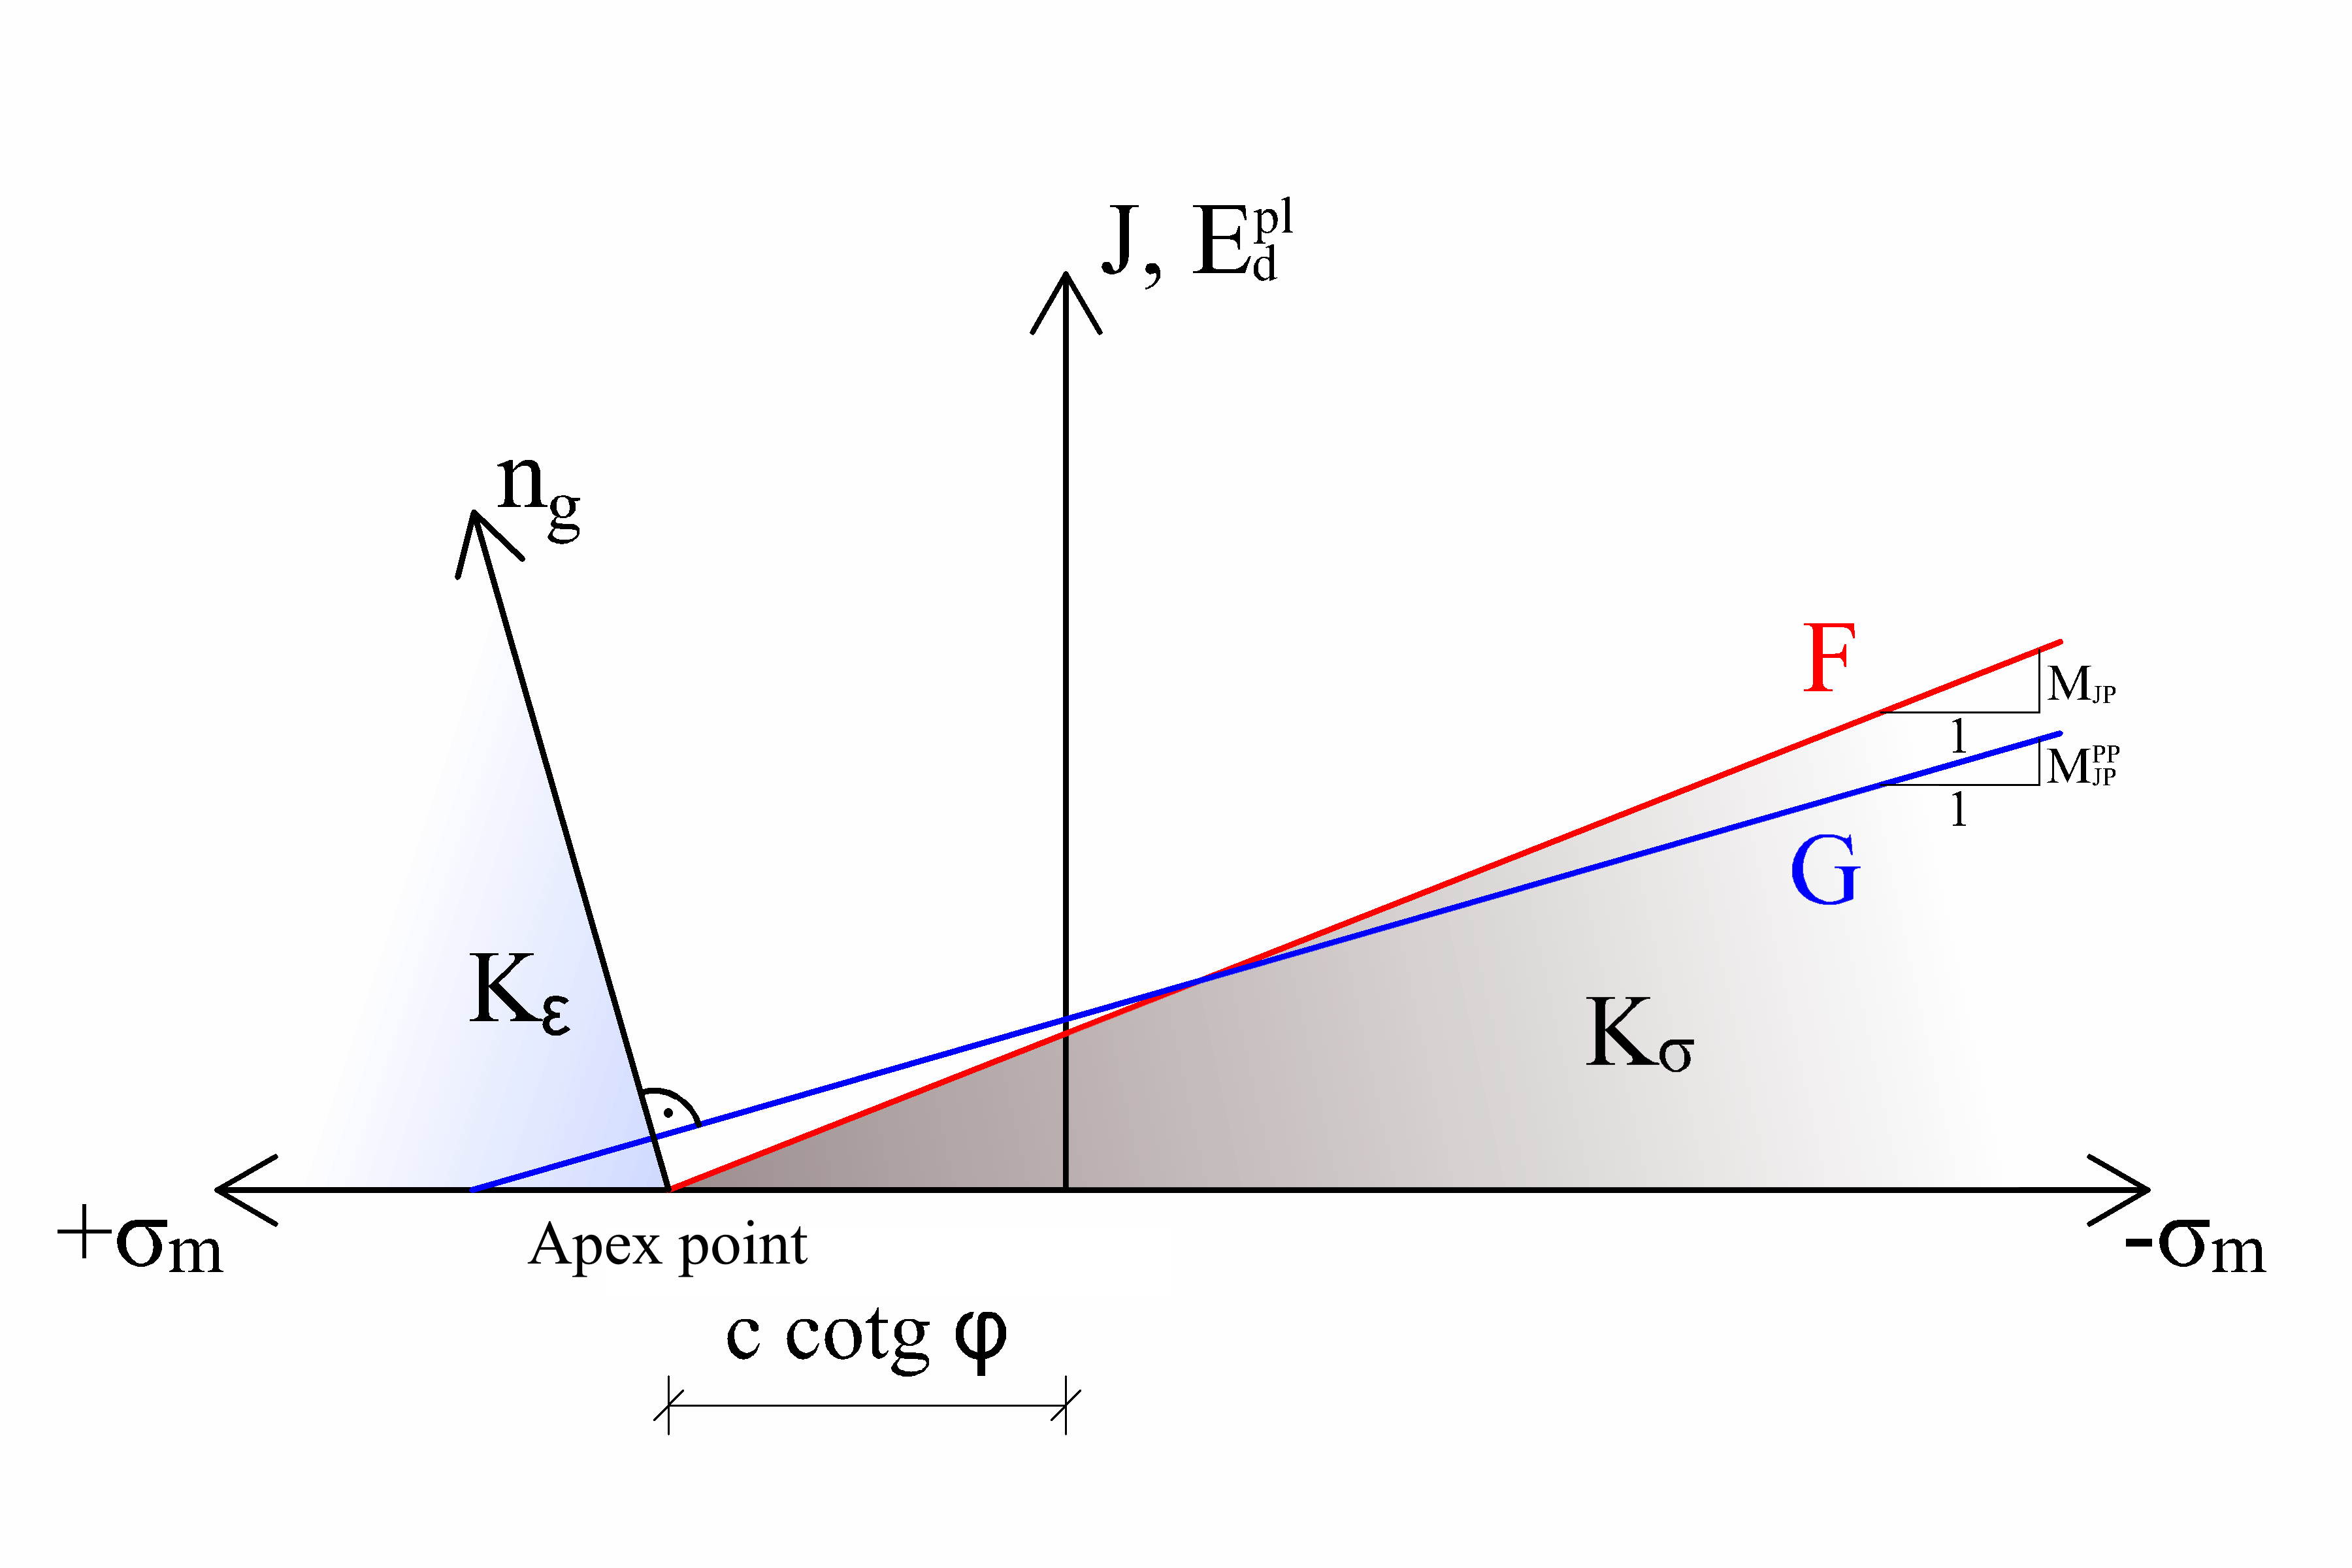
\includegraphics[width=0.8\textwidth, angle=0]{obrazky/apex_cones_my.png}
	\caption[Apex abmissible regions]{Apex admissible regions for stresses and plastic strain rates \cite{geofem}.} \label{obr:apex_cones}
\end{figure}

In the literature we can find two different stands for performing apex problem:

\begin{itemize}
	\item Return with constant material parameters.
	\item Return with hardening/softening material.
\end{itemize}
At the first case, stress point just return to the apex (Fig.\ref{obr:apex_cones}), so stress takes the form


\begin{equation}\label{eq:sigPL}
	\sigma^{i+1} = 3c^{i} \cot \varphi^{i} \textbf{m}.
\end{equation}
If the second approach is chosen, we can use two facts. The first is that material parameters $c$ and $\varphi$ are functions of $E_d^{pl}$. The second is that when returning to the apex point, elastic strain have only volumetric part so $\Delta E_d^{pl}$ can be determined at first, because it does not change. And if elastic strain have only volumetric part, deviatoric plastic strain vector is equal to the deviatoric increment strain vector. Then $\dd E_d^{pl}$ can be determined by the deviatoric strain measure, which has the form

\begin{equation}\label{eq:sig_i}
	\Delta E_d^{pl} = \sqrt{2\Delta e^{pl}_{ij}\Delta e^{pl}_{ij}}
\end{equation}
where $e^{pl}$ represent deviatoric plastic strain vector. As next, hardening of parameters $c$ and $\varphi$ follows Eqs. (\ref{eq:c}) and (\ref{eq:phi}) with current $E_d^{pl}$. Then the stress takes the form with updated $c$ and $\varphi$, similar to Eq. (\ref{eq:sigPL}), as

\begin{equation}
	\sigma^{i+1} = 3c^{i+1} \cot \varphi^{i+1} \textbf{m}.
\end{equation}


\subsection{Curing model}
\indent

Behavior of thermoset polymers is difficult to simulate due to a large number of variables. Instead of making one complex model we decided to achieve more realistic behavior of our model with two simpler models. First is for the mechanical response, as you can se above. The second is a curing model based on \cite{heinrich2012generation}, which is already implemented in MARS solver \cite{mars} and thus is utilized in the proposed approach based on the serial coupling of the models. 

This model simulates generation of heat during the curing of polymers. The curing of an epoxy is in fact exothermic chemical reaction, and degree of cure is often measured by placing small element into a digital scanning calorimeter, which is maintaining the sample at constant temperature and measures generated heat during the curing. The degree of cure is often defined by

\begin{equation}
	\phi(t) = \dfrac{H(t)}{H_r},
\end{equation}
where $H_r$ represent the total heat generated. That means $\phi(t)$ increases from $0$ to $1$ at fully cured state. Rate of heat generation per unit mass have the form

\begin{equation}
	r = \dv{(H_r\phi)}{t}.
\end{equation}
The curing process is defined by a kinetic equation 

\begin{equation}\label{eq:curing_process}
	\dv{\phi}{t} = f(T,\phi)
\end{equation}
where $T$ represents temperature and $f(T,\phi)\geq 0$ is represented by 

\begin{equation}\label{eq:temperature_function}
	d(T,\phi) = (k_1(T)+k_2(T()\phi^m)(1-\phi)^n,
\end{equation}

\begin{equation}
	k_1(T) = A_1 \exp \left(-\dfrac{\Delta E_1}{TR}\right),
\end{equation}

\begin{equation}
	k_2(T) = A_2 \exp \left( -\dfrac{\Delta E_2}{TR}\right),
\end{equation}
where $m$ and $n$ are constants, $R$ means the gas constant, $A_1$, respective $A_2$, are frequency like constants and $\Delta E_1$, respective $\Delta E_2$, represent activation energies. For more information about these constants see also \cite{heinrich2012generation}.
When the structural composite is cured, process of heat generation due to curing is affected by heat conduction due to the presence of an external surface or along fibers. This process can be described by the local form of the first law of thermodynamics as

\begin{equation} \label{eq:heat_conduct}
	\rho \dv{\epsilon}{t} = - \pdv{q_i}{\chi_i} + \rho r + \sigma_{ij} \dv{t}\varepsilon_{ij},
\end{equation}
where $\epsilon$ it the internal energy per unit mass, $\rho$ represent the current mass density, $q_i$ are the components of the heat flux vector, $r$ means the heat supply per unit mass, $\sigma_{ij}$ are the stress components and $\varepsilon_{ij}$ are the components of the infinitesimal strain tensor. 
The rate of mechanical work $\sigma_{ij}\dv{\varepsilon_{ij}}{t} $, is assumed to be negligible and the internal energy is assumed to be proportional to temperature, $e=cT$, where $c$ is the specific heat capacity. The heat flux vector is related to the temperature gradient by the Fourier law of heat conduction with the form

\begin{equation}\label{eq:furrier_heat}
	q_i = - \kappa \pdv{T}{\chi_i},
\end{equation}
where $\kappa$ is the thermal conductivity. It is possible that the thermal conductivity depends on the degree of cure and the temperature $\kappa = \kappa(T, \phi)$. The Eq. (\ref{eq:heat_conduct}) with (\ref{eq:curing_process}) and (\ref{eq:furrier_heat}) and the started assumptions becomes

\begin{equation}\label{eq:thermal_conductivity}
	\rho c \pdv{T}{t} = \pdv{\chi_i} \left( \kappa(T, \phi)  \pdv{T}{\chi_i} \right) + \rho H_r \pdv{\phi}{t}.
\end{equation}
 
 Eqs. (\ref{eq:curing_process}), (\ref{eq:temperature_function}) and (\ref{eq:thermal_conductivity}) are a system of coupled nonlinear partial differential equations for the partial distribution and time variation of temperature and degree of cure based on the energy consideration. 
 
 If the degree of cure is calculated, we can determine the evolution of the longitudinal modulus $M(\phi)$, the shear modulus $\mu(\phi)$ and the bulk modulus $K(\phi)$. According to \cite{heinrich2012generation} the evolution of these parameters can be written as:
 
 \begin{align}
 	\mu(\phi) &= \dfrac{1}{2} \dfrac{\beta_\mu ( \mu_f - \mu_s)}{\left(1+(\phi-1/2)^2 \beta_\mu^2\right) \arctan(1/2\beta_\mu))}, \\
 	M(\phi) &= \dfrac{1}{2} \dfrac{\beta_M ( M_f - M_s)}{\left(1+(\phi-1/2)^2 \beta_M^2\right) \arctan(1/2\beta_M))} + K_{liq}, \\
 	K(\phi) &= M(\phi) - \dfrac{4}{3}\mu(\phi),
 \end{align}
 where $\beta_\mu$ and $\beta_M$ are fitting constants, $\mu_s$, $\mu_f$, $M_s$ and $M_f$ are the start and final value of the measure shear and longitudinal moduli. The bulk modulus of the liquid epoxy have the form
 
 \begin{equation}
 	K_{liq} = K_{tot}(0) = M_{tot}(0),
 \end{equation} 
 where total moduli can be determined by an analytical functions:
 
 \begin{align}
 	\mu_{tot} &= \dfrac{\arctan((\phi-\frac{1}{2})\beta_\mu)}{\arctan(\dfrac{\beta_\mu}{2})}(\mu_f-\mu_s)+\left( \dfrac{\mu_f + \mu_s}{2} \right),\\
 	M_{tot} &= \dfrac{\arctan((\phi-\frac{1}{2})\beta_M)}{\arctan(\dfrac{\beta_M}{2})}(M_f-M_s)+\left( \dfrac{M_f + M_s}{2} \right).
 \end{align}
 
 \subsection{Complex material model}
 \indent
 
 For the simulation of thermosetting polymers and their response we choose the approach with two serially coupled models. The aforementioned curing model is employed to calculate the evolution of material properties utilized by the Drucker-Prager model. This model uses the modified material parameters and calculates current stress and strain in a current time.. This would affect model behavior and, hopefully, provide more realistic results than a simple Drucker-Prager model. Note that this thesis represents a preliminary study and it is expected that more complex mechanical model, e.g. Microplane M4, will be utilized to characterize the mechanical behavior in more details. However, only results without the coupling are shown hereafter to verify the proper implementation of involved material models.